\documentclass[10pt, journal, a4paper]{IEEEtran}

%%% PACKAGES
\usepackage[english]{babel}
\usepackage{amsmath}
\usepackage{amssymb}
\usepackage{graphicx}
\graphicspath{ {pictures/} }
\usepackage{booktabs}
\usepackage{tikz}
\usepackage{hyperref}
\usepackage[utf8]{inputenc}
%%% packages (end)

\setlength{\IEEEdlabelindent}{\parindent}

%%% META
\author{Edoardo Colombo}
\title{Extending Phoenix to Sphinx}
\date{\today}

%%% HYPERREF OPTIONS
\makeatletter
\hypersetup{
    colorlinks, linkcolor=black, urlcolor=black,
    pdftitle={\@title},
    pdfauthor={\@author},
}
\makeatother

\begin{document}

\maketitle
\begin{abstract}
Automatically Generated Domains are the basis of modern botnets communication infrastructures:
they allow a resilient and almost non-trackable way of sending messages from the botmaster to the
infected machines over the network. Previous works developed techniques whose caveats were using
privacy-protected DNS data and employing a supervised learning approach. Phoenix \cite{Lorenzo2013}
was the first tool that tried to solve both of the aforementioned issues: an unsupervised learning
clustering approach based on linguistic features, consuming public passive DNS traffic databases.
We want to improve this result by a) employing incremental clustering techniques, b) adding multilingual/multicharset support and c) employing different clustering algorithms.
\end{abstract}

  %%% INPUT
  %!TEX root = <../main.tex>

\section{Introduction}
\label{sec:introduction}
\PARstart{M}{odern} botnets rely on Automatically Generated Domains (AGDs) to build a resilient
command and control communication infrastructure between the infected machines and the controller.
Thousands of domain names are randomly generated by the machines, using an unpredictable seed (e.g.
Twitter top tweets), which makes unfeasible any possible forecast, even if the
random generator methodology is known.
The botmaster produces the domain names using the same algorithm and seed,
and temporarily registers just one or a few of them. Therefore there will be just a few if not
only one non NXDOMAIN DNS answer that will resolve the domain name to its IP address, the
botmaster IP address. Once the command sequence has been sent over the network, nothing is left in
the hands of the defenders.

As this technique produces a high volume of NXDOMAIN DSN traffic, previous works
focused their effort in this direction. However the deployment and testing in such
cases impose quite constraining requirements, mainly related to privacy issues.

Bilge \emph{et al.} \cite{Exposure} proposed \textsc{Exposure}, which is an analysis
technique that exploits malicious DNS traffic peculiarities via passive monitoring. The main
issue arises from the use of local DNS traffic, with all its privacy-related restrictions.

Sandeep \emph{et al.}\cite{Sandeep2010} were the first ones to explore the issue of AGDs,
producing a \emph{supervised} learning based tool that leverages the randomization of AGD names as opposed
to the lower entropy featured by Human Generated Domains (HGDs).

Schiavoni \emph{et al.}\cite{Lorenzo2013} introduced \textsc{Phoenix}, an \emph{unsupervised}
system to detect, fingerprint and label malicious AGDs, based on linguistic features,
analyzing the top-hierarchy DNS traffic via passive monitoring.

We want to start from \textsc{Phoenix}, exploring a few possible further developments.
The remainder of this document is structured as follows: Section~\ref{sec:previous_work}
explains how \textsc{Phoenix} works whilst in Section~\ref{sec:proposed_approach} we
propose our future contributions and how they could improve the previous obtained results.


% section introduction (end)

  \section{Phoenix}
\label{sec:previous_work}
\textsc{Phoenix} is divided into three main modules:
\begin{description}
  \item[\textbf{DGA Discovery Module}] \hfill \\ is responsible of separating AGDs from HGDs;
  \item[\textbf{DGA Detection Module}] \hfill \\ is responsible of labeling the AGDs, matching them
    to a specific DGA;
  \item[\textbf{Intelligence and Insights Module}] \hfill \\ aggregates, correlates and monitors the
    results of the other modules to extract meaningful insights~\cite{Lorenzo2013}.
\end{description}

In the next sections we shall briefly describe the DGA Discovery and the DGA Detection module.

\subsection{DGA Discovery Module} % (fold)
\label{ssub:dga_discovery_module}
This module is further divided into three steps.
\begin{description}[\leftmargin 0.5\parindent]
  \item[\textbf{AGD Filtering}] \hfill \\
    During this phase \textsc{Phoenix}, provided with a set of malicious domains,
    computes a four elements feature vector which exploits four linguistic characteristics
    to separate AGDs from HGDs;
  \item[\textbf{AGD Clustering}] \hfill \\
    It receives a set of possible AGDs from the previous step. Then, it tries to
    produce clusters based on the IPs the domains resolve to.
  \item[\textbf{DGA Fingerprinting}] \hfill \\
    It extracts from each previously discovered cluster five cluster features, in order
    to fingerprint the DGA, as to be able successively label unseen domains.
\end{description}
% subsubsection dga_discovery_module (end)

\begin{figure*}[h!tp]
  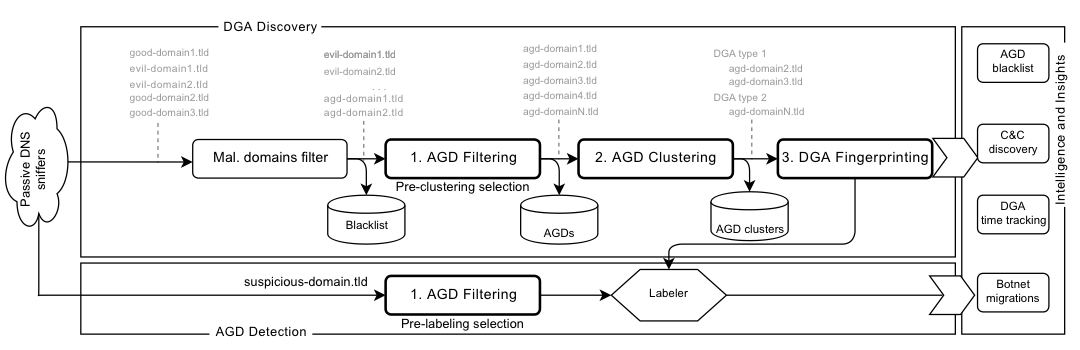
\includegraphics[width=\textwidth]{phoenix.png}
  \caption{The \textsc{Phoenix} modules.}
  \label{fig:phoenix}
\end{figure*}

\subsection{DGA Detection Module} % (fold)
\label{ssub:dga_detection_module}
The DGA Detection Module receives a previously unseen domain name. It determines
whether it is automatically or human generated, by running the filtering step of the
DGA Discovery Module. If this is the case, its features are computed and matched
against the fingerprints obtained before.
% subsubsection dga_detection_module (end)
% section previous_work (end)

  \section{Proposed Contributions}
\label{sec:proposed_approach}
We propose three further developments that could contribute to enhance the
effectiveness, the precision and the generality of \textsc{Phoenix}:
\begin{itemize}
  \item Incremental Clustering
  \item Multilingual/Multicharset Support
  \item Outliers detection
\end{itemize}
In the next paragraphs we shall discuss them thoroughly.

\subsection{Incremental Clustering} % (fold)
\label{sub:incremental_clustering}
So far \textsc{Phoenix} allows a \emph{batch} approach. The data must be crunched as
a whole, if new domain names are added to the dataset it is not possible to incrementally
update the obtained results. We want to integrate in our tool the techniques proposed in
\cite{Ning2010} and \cite{Chi2009} for incremental clustering, and we want to
substitute the Normalized Cuts technique for spectral clustering \cite{Shi2000} with
the more recent SPAN method developed by Shu \emph{et al.} \cite{Shu2011}.

% subsection incremental_clustering (end)

\subsection{Multilingual/Multicharset Support} % (fold)
\label{sub:multilingual_multicharset_support}
The linguistic features of \textsc{Phoenix} were extracted using the English
dictionary. We want to investigate the presence of other languages in malicious
domain names, e.g. Swedish or French. If we will find evidence of a substantial
presence of such languages, it is our intention to develop a multilingual module,
able to select correctly the dictionary to be used.

Moreover it is recently possible to use non-ASCII domain names, e.g.
www.$\pi$.com. This is an uncharted area that we want to explore as it might lead
to interesting results.

% subsection multilingual_multicharset_support (end)

\subsection{Outliers Detection} % (fold)
\label{sub:outliers_detection}
We want to investigate the possibility of using different clustering algorithms
(other than DBSCAN) to see if it leads to better performances. Especially it is of
our interest to search for an efficient technique for outliers detection purposes.

% subsection outliers_detection (end)

% section proposed_approach (end)

  \section{Conclusions}
\label{sec:conclusions_and_future_work}
\textsc{Phoenix} was a very interesting results in the study of botnets. We think that Schiavoni
\emph{et al.} identified a correct and interesting way of tackling the problem. We want to
continue on the same path, trying to improving and extending their work.

% section conclusions_and_future_work (end)

%%% sections (end)

\bibliographystyle{IEEEtran}
\bibliography{IEEEabrv,biblio}
\end{document}
